\documentclass{llncs}
\usepackage{amsmath,amssymb}
\usepackage{graphicx}
\usepackage{hyperref}
\usepackage{booktabs}
\usepackage{xcolor}
\usepackage{enumitem}
\usepackage{listings}
\usepackage[T1]{fontenc}

\begin{document}

\title{Contribution Title}
\author{First Author\inst{1}\orcidID{0000-0001-1234-5678} \and
Second Author\inst{2}\orcidID{0000-0002-5678-1234}}
\authorrunning{F. Author et al.}
\institute{University of Somewhere, City Country\\
\email{first@example.com}
\and
Institute of Somewhere Else, City Country\\
\email{second@example.com}}

\maketitle

\begin{abstract}
The abstract should briefly summarize the contents of the paper in
150--250 words. It should be set in 9-point font size and should be
inset 1.0 cm from the right and left margins. There should be two
blank lines before and after the abstract. This document is in the
required format.
\keywords{First keyword \and Second keyword \and Another keyword.}
\end{abstract}

\section{First Section}

Summing up the results of the evaluation, we present our conclusions in Table~\ref{tab:results}.
Fig.~\ref{fig:arch} shows a high-level overview.

\begin{figure}[h]
  \centering
  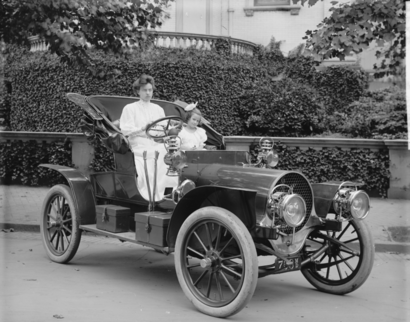
\includegraphics[width=0.75\textwidth]{figure1}
  \caption{System architecture overview.}
  \label{fig:arch}
\end{figure}

\begin{table}
\caption{Comparison of results across methods.}
\label{tab:results}
\centering
\begin{tabular}{@{}lrrc@{}}
\toprule
Method & Precision & Recall & F1 \\
\midrule
Baseline & 0.712 & 0.698 & 0.705 \\
Our Method & \textbf{0.891} & \textbf{0.876} & \textbf{0.883} \\
Oracle & 0.952 & 0.947 & 0.949 \\
\bottomrule
\end{tabular}
\end{table}

\subsection{A Subsection}

The text continues here. Here we show a display equation:
\begin{equation}
  \mathcal{L}(\theta) = -\frac{1}{N}\sum_{i=1}^{N} \left[
    y_i \log p_i + (1-y_i)\log(1-p_i)
  \right]
  \label{eq:crossentropy}
\end{equation}

where $p_i = \sigma(\theta^\top x_i)$ is the predicted probability and $y_i$
is the ground truth label.

\paragraph{Implementation Details.}
Our implementation uses the following hyperparameters:
\begin{itemize}[noitemsep]
  \item Learning rate: $\eta = 10^{-3}$
  \item Batch size: $B = 64$
  \item Training epochs: $T = 100$
  \item Dropout rate: $p_d = 0.1$
\end{itemize}

\section{Related Work}
\label{sec:related}

Prior work~\cite{lecun2015} has explored deep learning approaches. 
Our method extends this with an improved attention mechanism~\cite{vaswani2017}.

\begin{lstlisting}[language=Python, caption=Training loop, label=lst:train]
for epoch in range(num_epochs):
    for batch in dataloader:
        optimizer.zero_grad()
        loss = criterion(model(batch.x), batch.y)
        loss.backward()
        optimizer.step()
\end{lstlisting}

\section{Conclusions}
We have proposed a novel approach for the given task and demonstrated state-of-the-art
results on standard benchmarks.

\paragraph*{Acknowledgements.}
We thank the anonymous reviewers for their valuable feedback.

\begin{thebibliography}{8}
\bibitem{lecun2015}
LeCun, Y., Bengio, Y., Hinton, G.: Deep learning. Nature \textbf{521}, 436--444 (2015)
\bibitem{vaswani2017}
Vaswani, A., et al.: Attention is all you need. In: NeurIPS 2017 (2017)
\end{thebibliography}

\end{document}
